\input{/home/nick/latex-preambles/xelatex.tex}

\newcommand{\imagesPath}{.}

\title{
	\textbf{Δίκτυα Υπολογιστών} \\~\\
	Εργαστηριακή Άσκηση 7 \\ 
	Πρωτόκολλα TCP και UDP
}
\author{}
\date{}

\begin{document}
	\maketitle
	
	\begin{tabular}{|l|l|}
		\hline
		\textbf{Ονοματεπώνυμο:} Νικόλαος Παγώνας, el18175 & \textbf{Ομάδα:} 4 (Τρίτη εξ' αποστάσεως) \\
		\hline
		\textbf{Όνομα PC/ΛΣ:} nick-ubuntu/Ubuntu 20.04.3 LTS & \textbf{Ημερομηνία:} Τρίτη 30/11/2021\\
		\hline
		\textbf{Διεύθυνση IP:} \verb|192.168.1.15| & \textbf{Διεύθυνση MAC:} \verb|3c:2c:30:e1:1c:55|\\
		\hline
	\end{tabular}

	\section*{1. Μετάδοση δεδομένων με TCP}
		
		\subsection*{1.1} 
			Χρησιμοποιήσαμε το φίλτρο \verb|host 192.168.1.15|.
		
		\subsection*{1.2} 
			Η σύνταξη του φίλτρου είναι: \\
		 	\verb+ip.dst == 1.1.1.1 || ip.dst == 2.2.2.2 || ip.dst == 147.102.40.1+
		
		\subsection*{1.3} 
			Προσπαθεί να συνδεθεί στην θύρα 23.
		
		\subsection*{1.4} 
			Η σύνταξη του φίλτρου είναι \verb|tcp.port == 23|.
		
		\subsection*{1.5} 
			Ενεργοποιείται η σημαία SYN.
		
		\subsection*{1.6} 
			Κάνει 7 προσπάθειες και στις δύο περιπτώσεις.
		
		\subsection*{1.7} 
			Παρατηρούμε ότι ο χρόνος μεταξύ δύο διαδοχικών προσπαθειών επανασύνδεσης μεγαλώνει εκθετικά (1, 2, 4, 8, 16, 32 sec).
		
		\subsection*{1.8} 
			Τα αποτελέσματα μοιάζουν πολύ μεταξύ των δύο περιπτώσεων.
		
		\subsection*{1.9} 
			Παρατηρήσαμε μόνο το πρώτο βήμα της τριπλής χειραψίας.
		
		\subsection*{1.10} 
			Ο υπολογιστής μας απλώς εγκαταλείπει την προσπάθεια.
		
		\subsection*{1.11} 
			Η σύνταξη του φίλτρου είναι \verb|tcp.port == 23 && ip.addr == 147.102.40.1|.
		
		\subsection*{1.12} 
			Ο υπολογιστής μας κάνει μόνο μία προσπάθεια.
		
		\subsection*{1.13}
			Σε σύγκριση με το ερώτημα 1.8:
			\begin{itemize}
				\item Ο υπολογιστής κάνει μόνο μία προσπάθεια, ενώ πριν έκανε 7 προσπάθειες
				\item Ο υπολογιστής λαμβάνει απάντηση, ενώ πριν δεν έλαβε.
			\end{itemize}
		
		\subsection*{1.14} 
			Περιλαμβάνει τις σημαίες: 
			
			\begin{itemize}
				\item Reserved: 0 (3 bits δεσμευμένα για μελλοντική χρήση, πρέπει να έχουν την τιμή 000)
				\item Nonce: 0
				\item Congestion Window Reduced (CWR): 0
				\item ECN-Echo: 0
				\item Urgent: 0
				\item Acknowledgment: 1
				\item Push: 0
				\item Reset: 1
				\item Syn: 0
				\item Fin: 0
			\end{itemize}
			
		
		\subsection*{1.15} 
			Η σημαία Reset.
		
		\subsection*{1.16} 
			Το μέγεθος της επικεφαλίδας είναι 20 bytes και το μέγεθος των δεδομένων είναι 0 bytes.
		
		\subsection*{1.17} 
			\begin{itemize}
				\item Source Port: 16 bits
				\item Destination Port: 16 bits
				\item Sequence Number: 32 bits
				\item Acknowledgment Number: 32 bits
				\item Header Length (ή Data Offset): 4 bits
				\item Reserved: 3 bits
				\item Flags: 9 bits
				\item Window: 16 bits
				\item Checksum: 16 bits
				\item Urgent Pointer: 16 bits 
			\end{itemize}
		
		\begin{figure}[H]
			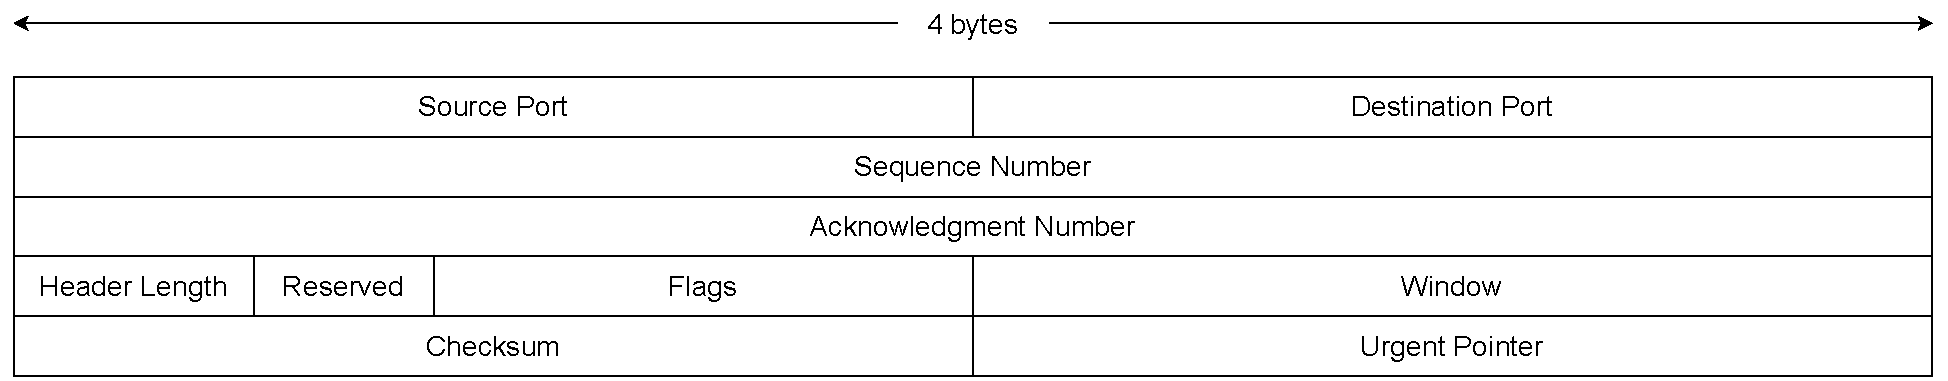
\includegraphics[width=\linewidth]{\imagesPath/1.17.pdf}
		\end{figure}
		
		\subsection*{1.18}
			Το πεδίο που καθορίζει το μέγεθος επικεφαλίδας είναι το Data Offset. Το Wireshark χρησιμοποιεί την ονομασία Header Length.
		
		\subsection*{1.19} 
			Η τιμή του Header Length δείχνει το μήκος του TCP Header σε λέξεις των 32 bit (4 byte). Επομένως για Header Length = 5, έχουμε μήκος επικεφαλίδας $5 \cdot 4 = 20$ bytes.
		
		\subsection*{1.20} 
			Όχι, δεν υπάρχει.
		
		\subsection*{1.21} 
			Το μήκος τεμαχίου προκύπτει αν από το Total Length του IPv4 πακέτου αφαιρέσουμε το Header Length του IPv4 πακέτου και το Header Length του TCP τεμαχίου, δηλαδή:
			
			\[
				\text{Μήκος τεμαχίου TCP} = \text{Συνολικό Μήκος IP Πακέτου} - (\text{Μήκος Επικεφαλίδας IP} + \text{Μήκος Επικεφαλίδας TCP}) 
			\]
		
		\subsection*{1.22} 
			Είναι 40 bytes.
			
		\subsection*{1.23}
			Υπάρχει διαφορά η οποία οφείλεται στο πεδίο Options (20 bytes) του πακέτου TCP που αποστέλλεται από τον υπολογιστή μας. Τα Options περιέχουν τις απαραίτητες πληροφορίες για την εγκατάσταση της σύνδεσης.
			
	\section*{2. Εγκατάσταση σύνδεσης, μεταφορά δεδομένων και απόλυση σύνδεσης TCP}
		
		\subsubsection*{2.1} 
			Χρησιμοποιήσαμε το φίλτρο \verb|host edu-dy.cn.ntua.gr|
		
		\subsection*{Έγκατάσταση σύνδεσης}
		
		\subsubsection*{2.2} 
			Προσπαθεί να συνδεθεί στη Θύρα 21.
			
		
		\subsubsection*{2.3} 
			Με τη θύρα 20.
		
		\subsubsection*{2.4} 
			Η σύνταξη του φίλτρου είναι \verb|tcp.port == 21|.
		
		\subsubsection*{2.5} 
			Ανταλλάσσονται 3 τεμάχια.
		
		\subsubsection*{2.6} 
			Χρησιμοποιούνται οι σημαίες SYN και ACK.
		
		\subsubsection*{2.7} 
			Το μέγεθος των επικεφαλίδων είναι 40, 40 και 32 bytes αντίστοιχα.
		
		\subsubsection*{2.8} 
			Το μέγεθος των δεδομένων είναι 0 bytes.
		
		\subsubsection*{2.9} 
			Διαρκεί 0.010129281 sec.
		
		\subsubsection*{2.10} 
			Ναι, συμφωνεί.
		
		\subsubsection*{2.11} 
			Η πλευρά του υπολογιστή μας (192.168.1.15) ανακοινώνει Sequence Number (raw) ίσο με 4233096794, ενώ η πλευρά του edu-dy.cn.ntua.gr (147.102.40.15) ανακοινώνει Sequence Number (raw) ίσο με 2513291583.
		
		\subsubsection*{2.12} 
			Προκύπτει από το Sequence Number (raw) του τελευταίου τεμαχίου που ελήφθη προσαυξημένο κατά 1.
			
		\subsubsection*{2.13} 
			Το Sequence Number (raw) προκύπτει από το προηγούμενο Sequence Number του ίδιου κόμβου προσαυξημένο κατά 1, ενώ το Acknowledgment Number (raw) προκύπτει από το Sequence Number του τελευταίου τεμαχίου που ελήφθη προσαυξημένο κατά 1.
		
		\subsubsection*{2.14} 
			Το μήκος δεδομένων των τεμαχίων της τριπλής χειραψίας είναι ίσο με 0.
		
		\subsubsection*{2.15} 
			Επειδή τόσο ο αριθμός σειράς όσο και ο αριθμός επιβεβαίωσης έχουν μέγεθος 4 bytes (32 bit), η μέγιστη τιμή που μπορούν να πάρουν και οι δύο είναι $2^{32}-1=4.294.967.295$.
			
		\subsubsection*{2.16} 
			Θα εφαρμόσουμε το φίλτρο: \\
			\verb+tcp.port == 21 && tcp.len == 0 && ((tcp.seq == 0) || (tcp.seq == 1 && tcp.ack == 1))+
			
		\subsubsection*{2.17} 
			Ο υπολογιστής μας ανακοινώνει παράθυρο 64240 bytes ενώ ο server ανακοινώνει παράθυρο 65535 bytes.
		
		\subsubsection*{2.18} 
			Η σχετική πληροφορία μεταφέρεται στο πεδίο Window.
		
		\subsubsection*{2.19} 
			Το μικρότερο μέγεθος παραθύρου που παρατηρούμε είναι 502 bytes ενώ το μεγαλύτερο είναι 65535 bytes.
		
		\subsubsection*{2.20} 
			Ανακοινώνει την τιμή των 1460 bytes.
		
		\subsubsection*{2.21} 
			Η τιμή αυτή προκύπτει ως εξής: 
			
			\[
				\text{MSS} = \text{MTU} - (\text{IPv4 Header Length} + \text{TCP Header Length}) = \text{MTU} - 40 = 1500 - 40 = 1460.
			\]
		
		\subsubsection*{2.22} 
			Η τιμή του MSS μεταφέρεται στο πεδίο Options, και συγκεκριμένα σε ένα Option που ονομάζεται "TCP Option - Maximum segment size", το οποίο περιέχει ένα πεδίο "MSS Value".
			
		\subsubsection*{2.23} 
			Ο edu-dy.cn.ntua.gr ανακοινώνει τιμή MSS = 536. 
			
		\subsubsection*{2.24} 
			Και πάλι έχουμε:
			
			\[
				\text{MSS} = \text{MTU} - 40 = 576 - 40 = 536.
			\]
				
		\subsubsection*{2.25} 
			Το μέγεθος του μεγαλύτερου τεμαχίου TCP είναι ίσο με το MSS που ανακοινώνει ο server στον υπολογιστή μας, μαζί με το μέγεθος της επικεφαλίδας TCP, δηλαδή 536 + 20 = 556 bytes.
		
		\subsection*{Απόλυση σύνδεσης}
		
		\subsubsection*{2.26} 
			Ενεργοποιείται η σημαία FIN.
		
		\subsubsection*{2.27} 
			Η σύνταξη του φίλτρου είναι \verb|tcp.flags.fin == 1|.
					
		\subsubsection*{2.28} 
			Η διαδικασία απόλυσης εκκινεί ανεξάρτητα και από τις δύο πλευρές (half close). Σε αυτή την καταγραφή, το πακέτο με σημαία FIN το στέλνει πρώτος ο server (και μετά από 1 msec περίπου ακολουθεί και ο υπολογιστής μας).
		
		\subsubsection*{2.29} 
			Ανταλλάσσονται συνολικά 4 τεμάχια.
		
		\subsubsection*{2.30} 
			Και τα 4 τεμάχια έχουν μέγεθος επικεφαλίδας 32 bytes.
		
		\subsubsection*{2.31} 
			Και τα 4 τεμάχια έχουν μέγεθος δεδομένων 0 bytes.
		
		\subsubsection*{2.32} 
			\begin{align*}
				& \text{Συνολικό μήκος πακέτου IPv4} = \\
				& = \text{Μέγεθος IPv4 επικεφαλίδας} + \text{Μέγεθος TCP επικεφαλίδας} + \text{Μέγεθος Δεδομένων} = \\
				& = 20 \text{ bytes} + 32 \text{ bytes} + 0 \text{ bytes} = \textbf{52 bytes.}
			\end{align*}
		
		\subsubsection*{2.33} 
			Η αιτιολόγηση είναι πανομοιότυπη με το ερώτημα 2.32.
		
		\subsubsection*{2.34} 
			Από την πλευρά του υπολογιστή μας μεταφέρθηκαν 103 bytes, ενώ από την πλευρά του server μεταφέρθηκαν 375 bytes.
		
		\subsubsection*{2.35} 
			Προσδιορίσαμε το πλήθος τους με βάση το Relative Sequence Number.
		
		\subsection*{Μεταφορά δεδομένων}
		
		\subsubsection*{2.36}
			Η σύνταξη του φίλτρου είναι \verb|tcp.port == 20|.
		
		\subsubsection*{2.37} 
			Η πλευρά του υπολογιστή μας ανακοινώνει MSS = 1460, ενώ η πλευρά του server ανακοινώνει MSS = 536.
		
		\subsubsection*{2.38} 
			Το μέγεθος του μεγαλύτερου τεμαχίου TCP (συμπεριλαμβανομένης και της επικεφαλίδας TCP) είναι 1480 bytes.
		
		\subsubsection*{2.39} 
			Είναι 0.005052912 sec (\char`\~5 msec).
		
		\subsubsection*{2.40} 
			Ο υπολογιστής μας στέλνει επιβεβαίωση ανά \char`\~2-3 τεμάχια.
		
		\subsubsection*{2.41} 
			Ναι, η τιμή του παραθύρου αλλάζει, με την μικρότερη τιμή να είναι 488 bytes.

		\subsubsection*{2.42} 
			\begin{itemize}
				\item Μέγεθος πλαισίου: 1114 bytes
				\item Μήκος επικεφαλίδας Ethernet: 14 bytes
				\item Μήκος επικεφαλίδας IP: 20 bytes
				\item Μήκος επικεφαλίδας TCP: 32 bytes
			\end{itemize}
		
		\subsubsection*{2.43} 
			Είναι αναμενόμενη αφού είναι μικρότερη από το μέγιστο που μπορεί να δεχθεί ο υπολογιστής μας.
		
		\subsubsection*{2.44}
			Σε αυτή την περίπτωση προφανώς θα είχαμε θρυμματισμό.
		 
		\subsubsection*{2.45} 
			Μεταδόθηκαν συνολικά 61442 bytes από την μεριά του server και 1 byte από την μεριά του υπολογιστή μας.
		
		\subsubsection*{2.46} 
			Ο ρυθός μεταφοράς δεδομένων ήταν 992 kbyte/sec.
		
		\subsubsection*{2.47} 
			Δεν υπήρξαν αναμεταδόσεις, αφού δεν υπάρχουν δύο τεμάχια με ίδιο Sequence Number.

	\section*{3. Αποφυγή συμφόρησης στο TCP}
		
		\subsection*{3.1} 
			Η σύνταξη του φίλτρου είναι \verb|tcp.port == 20|.

		\subsection*{3.2} 
			Η διεύθυνση του υπολογιστή που κατέβασε το αρχείο PCATTCP.exe είναι η 94.65.141.44.

		\subsection*{3.3} 
			Το RTT είναι 0.014626 sec (\char`\~14.6 msec), τιμή αρκετά μεγαλύτερη από αυτή που βρήκαμε στο ερώτημα 2.39.

		\subsection*{3.4} 
			Παρατηρώ ότι κάθε φορά στέλνονται όλο και περισσότερα τεμάχια μαζεμένα. Αυτό συμβαίνει διότι ο edu-dy.cn.ntua.gr λαμβάνει διαδοχικά ACK, και άρα μεγαλώνει το μέγεθος παραθύρου.

		\subsection*{3.5} 
			Ο edu-dy.cn.ntua.gr έστειλε 4 τεμάχια στο πρώτο RTT, που είναι σύμφωνο με την παράγραφο 3.1 του RFC 5681.

		\subsection*{3.6}
			Κατά το δεύτερο και τρίτο RTT έστειλε 6 και 10 τεμάχια αντίστοιχα, επειδή μετά από κάθε ACK μεγαλώνει και το μέγεθος του παραθύρου.
		
		\subsection*{3.7}
			Ναι, το διάγραμμα είναι παρόμοιο.
	
	\section*{4. Μετάδοση δεδομένων με UDP}
		
		\subsection*{4.1}
			Η σύνταξη του φίλτρου σύλληψης που χρησιμοποιήσαμε είναι \verb|udp|.

		\subsection*{4.2}
			\begin{itemize}
				\item Source Port: 2 bytes
				\item Destination Port: 2 bytes
				\item Length: 2 bytes
				\item Checksum: 2 bytes
			\end{itemize}

		\subsection*{4.3}
			Το συνολικό μέγεθος της επικεφαλίδας UDP είναι 8 bytes.

		\subsection*{4.4}
			Το μήκος του συγκεκριμένου δεδομενογράμματος είναι 43 bytes.

		\subsection*{4.5}
			 Το Length εκφράζει το συνολικό μήκος του δεδομενογράμματος.

		\subsection*{4.6}
			Το ελάχιστο μέγεθος ενός δεδομενογράμματος UDP είναι μόνο η επικεφαλίδα, δηλαδή 8 bytes. Το μέγιστο μέγεθος είναι $65535-20 = 65515$ bytes, αφού το μέγιστο μέγεθος ενός IPv4 πακέτου είναι 65535 bytes.

		\subsection*{4.7}
			Το μέγιστο μήκος πακέτου που μπορεί να σταλεί και παραληφθεί με βεβαιότητα είναι 516 bytes, αφού η επικεφαλίδα IPv4 μπορεί να φτάσει δυνητικά και τα 60 bytes.

		\subsection*{4.8}
			Δεν παρατηρήσαμε άλλα πρωτόκολλα πέραν του DNS.

		\subsection*{4.9}
			Η σύνταξη του φίλτρου απεικόνισης που χρησιμοποιήσαμε είναι \verb|dns|.

		\subsection*{4.10}
			Η διεύθυνση IPv4 του εξυπηρετητή DNS είναι 192.168.1.1 (ίδια με του router μας).

		\subsection*{4.11}
			\begin{itemize}
				\item Source Port: 38729
				\item Destination Port: 53
			\end{itemize}

		\subsection*{4.12}
			\begin{itemize}
				\item Source Port: 53
				\item Destination Port: 38729
			\end{itemize}
		
		\subsection*{4.13}
			Η θύρα που αντιστοιχεί στο πρωτόκολλο εφαρμογής DNS είναι η 53.
\end{document}